\section{Introdução}\label{introduuxe7uxe3o}

\begin{frame}{Introdução}

\begin{figure}[h]
    
\includegraphics[scale=0.5]{img/webrtc-logo-horiz-retro-750x140.png}
\end{figure}

\textbf{WebRTC} é um projeto livre que fornece a navegadores web e
aplicações mobile capacidade de \textbf{Real-Time Communications}
(Comunicação em tempo real) através de \emph{API}s simples.

\end{frame}

\begin{frame}{Introdução}

É uma iniciativa da W3C em conjunto com Google, Mozilla and Opera, entre
outros.

O Web Real-Time Communications Working Group foi criado para criar e
gerenciar os padrões do WebRTC.

\end{frame}

\begin{frame}{Aplicação}

Pode ser aplicado para todo tipo de plataforma que requer comunicação de
alta qualidade na web, tais como troca de \textbf{mensagens} e
transferência de \textbf{arquivos}, componentes de \textbf{áudio e
vídeo} para vídeo conferências, \textbf{comunicação e controle} de
equipamentos IoT.

\begin{figure}[h]
    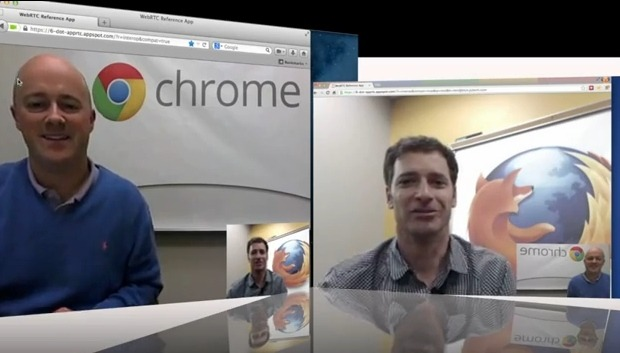
\includegraphics[scale=0.35]{img/firefox-chrome-webrtc.jpg}
\end{figure}

\end{frame}

\section{Arquitetura}\label{arquitetura}

\begin{frame}{Arquitetura}

A nível de browser:

\begin{figure}[h]
    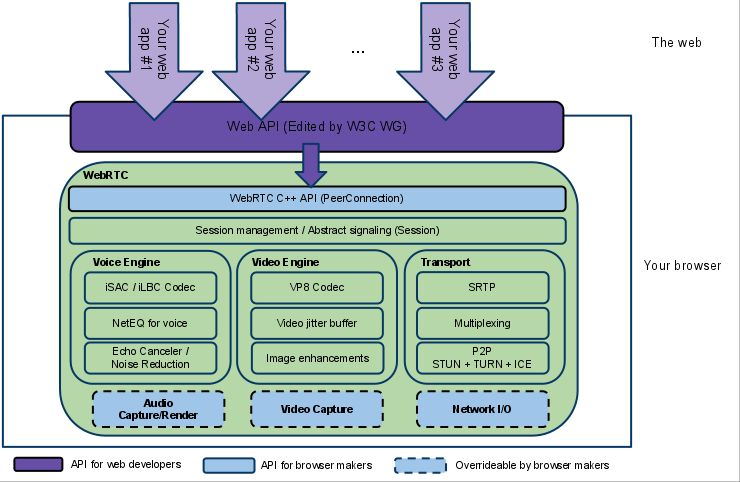
\includegraphics[scale=0.35]{img/webrtc-architecture.png}
\end{figure}

\end{frame}

\begin{frame}{Arquitetura}

WebRTC permite comunicação peer-to-peer (P2P) entre browsers

MAS ainda são necessários \textbf{servidores}:

\bigskip

\textbf{Para que clientes possam trocar metadados para coordenar a
comunicação - isto é chamado de \emph{Signaling}.}

\bigskip

\textbf{Para lidar com \emph{NAT}s (Network Address Translators) e
\emph{Firewalls}.}

\end{frame}

\begin{frame}{Arquitetura}

\begin{figure}[h]
    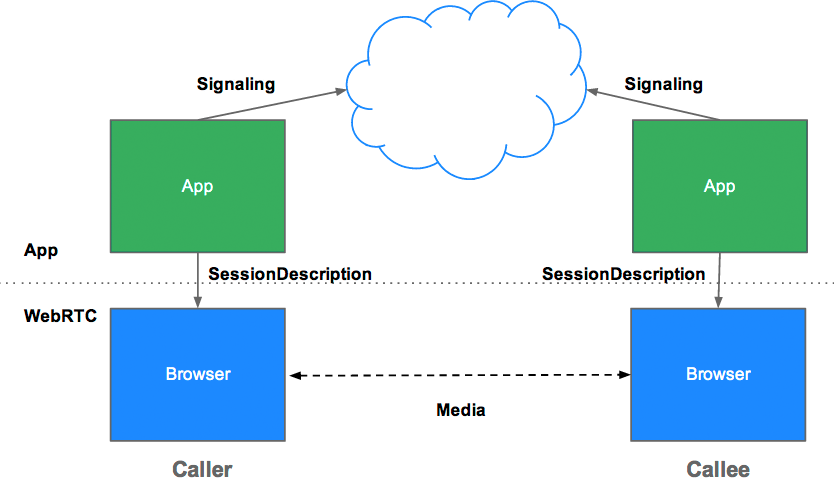
\includegraphics[scale=0.35]{img/jsep.png}
\end{figure}

\end{frame}

\begin{frame}{Arquitetura}

Para evitar redundância e maximizar a compatibilidade com tecnologias já
estabelecidas, métodos e protocolos para fazer \emph{Signaling} não
foram especificados pelos padrões do WebRTC.

A lógica por trás disso é que diferentes aplicações podem preferir
utilizar diferentes protocolos, tais como \emph{SIP} (Session Initiation
Protocol - VoIP) ou \emph{Jingle} (extensão do XMPP/Jabber - Troca de
mensagens de texto) como protocolos para fazer \emph{Signaling}.

\end{frame}
